\documentclass[a4paper]{article}

%% Language and font encodings
\usepackage[english]{babel}
\usepackage[utf8x]{inputenc}
\usepackage[T1]{fontenc}

%% Sets page size and margins
\usepackage[a4paper,top=3cm,bottom=2cm,left=3cm,right=3cm,marginparwidth=1.75cm]{geometry}

%% Useful packages
\usepackage{amsmath}
\usepackage{graphicx}
\usepackage{enumitem}
\usepackage[colorinlistoftodos]{todonotes}
\usepackage[colorlinks=true, allcolors=blue]{hyperref}

\graphicspath{ {images/} }
\newcommand{\true}{$T$}
\newcommand{\false}{$F$}
\newcommand{\ans}{\textit{Answer: }}
\newcommand{\prf}{\textbf{Proof:}}
\newenvironment{question}[2][Question]{\begin{trivlist}
\item[\hskip \labelsep {\bfseries #1}\hskip \labelsep {\bfseries #2.}]}{\end{trivlist}}

\title{CS251 Sample Midterm Answers}
\author{Elnard Utiushev}

\begin{document}

\maketitle

\textbf{Please use issues tab to report any mistakes.}

\section*{Part I. True-False and Multiple-Choice Questions}
\begin{enumerate}
  \item $\sum_{i=1}^{n}i^2$ is $\Theta(n^3)$ \\
  \textbf{True} \\
  \ans 
  $$\sum_{i=1}^{n}i^2 = \frac{n(n+1)(2n+1)}{6}$$
  \begin{center}
    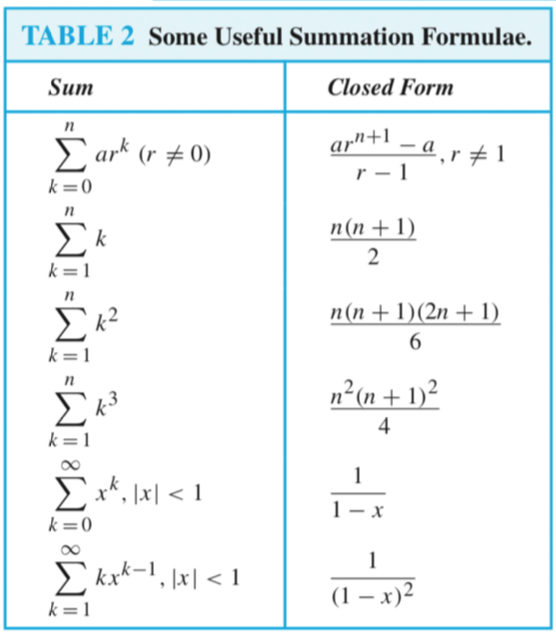
\includegraphics[width=0.5\textwidth]{fig1.png}
    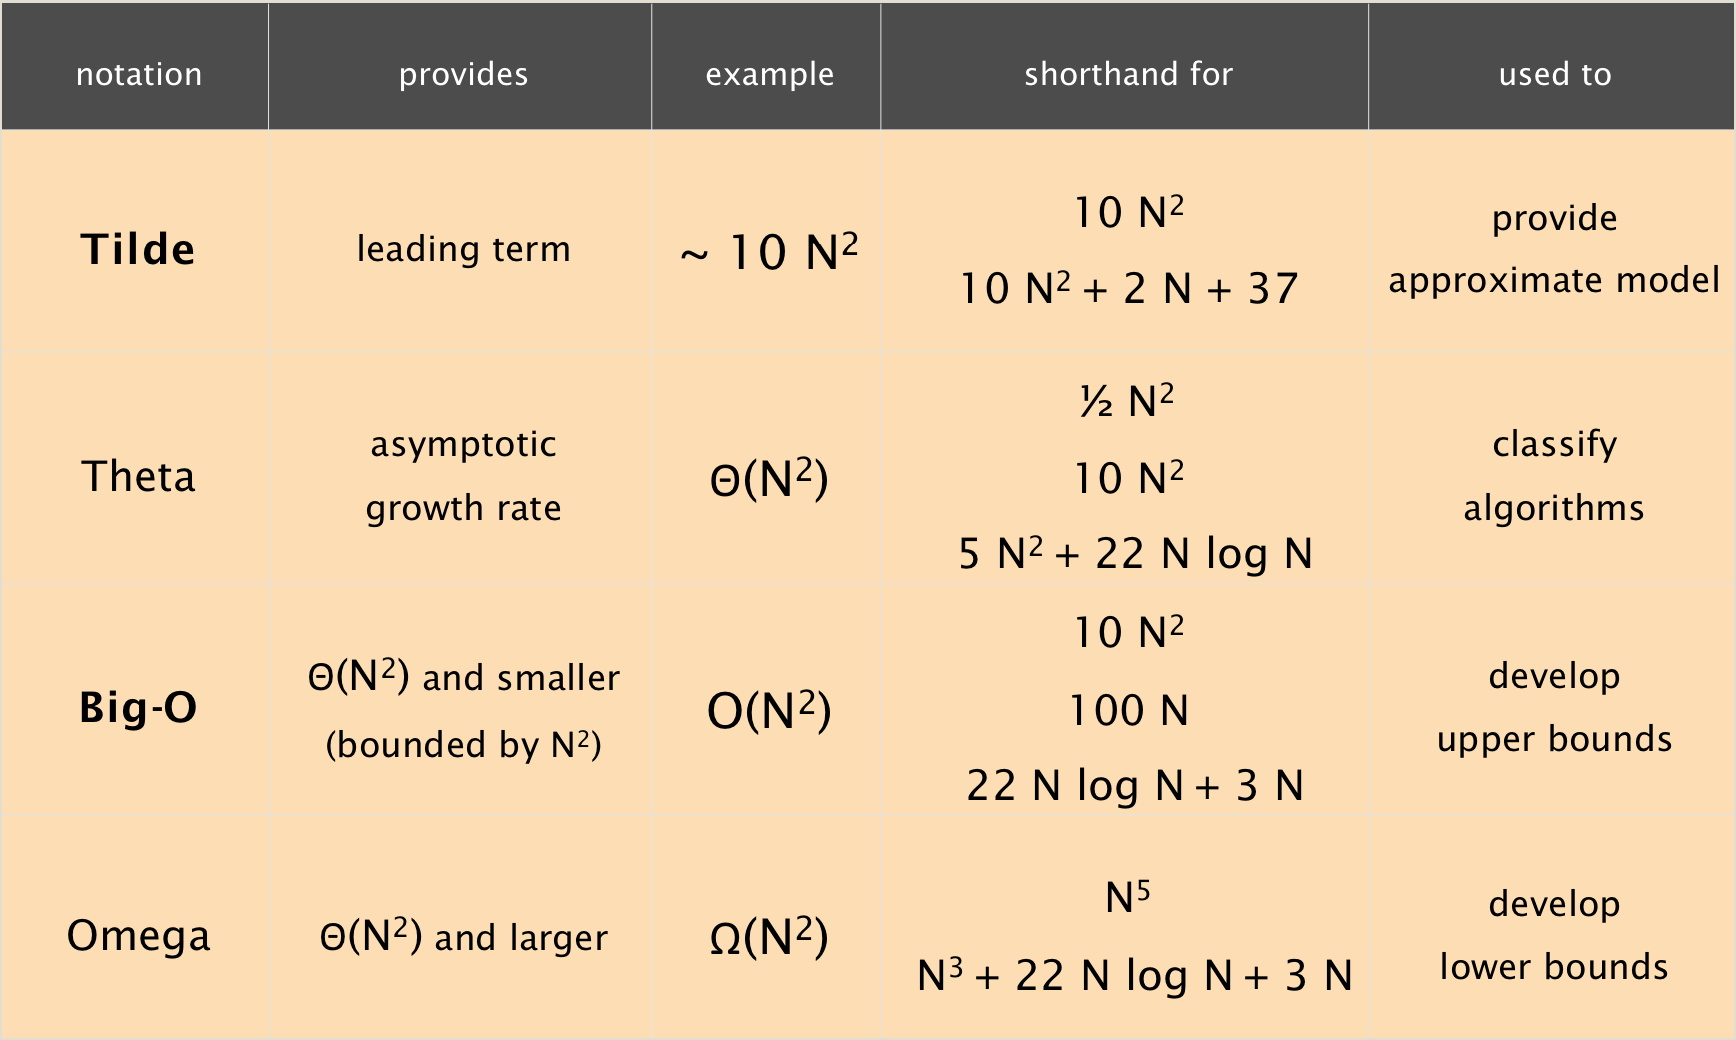
\includegraphics[width=0.8\textwidth]{fig2.png}
  \end{center}

  \item The worst-case number of comparisons used by Merge Sort to sort $n$ elements is
  O($n$ log $n$). \\
  \textbf{True} \\
  \ans
  \begin{center}
    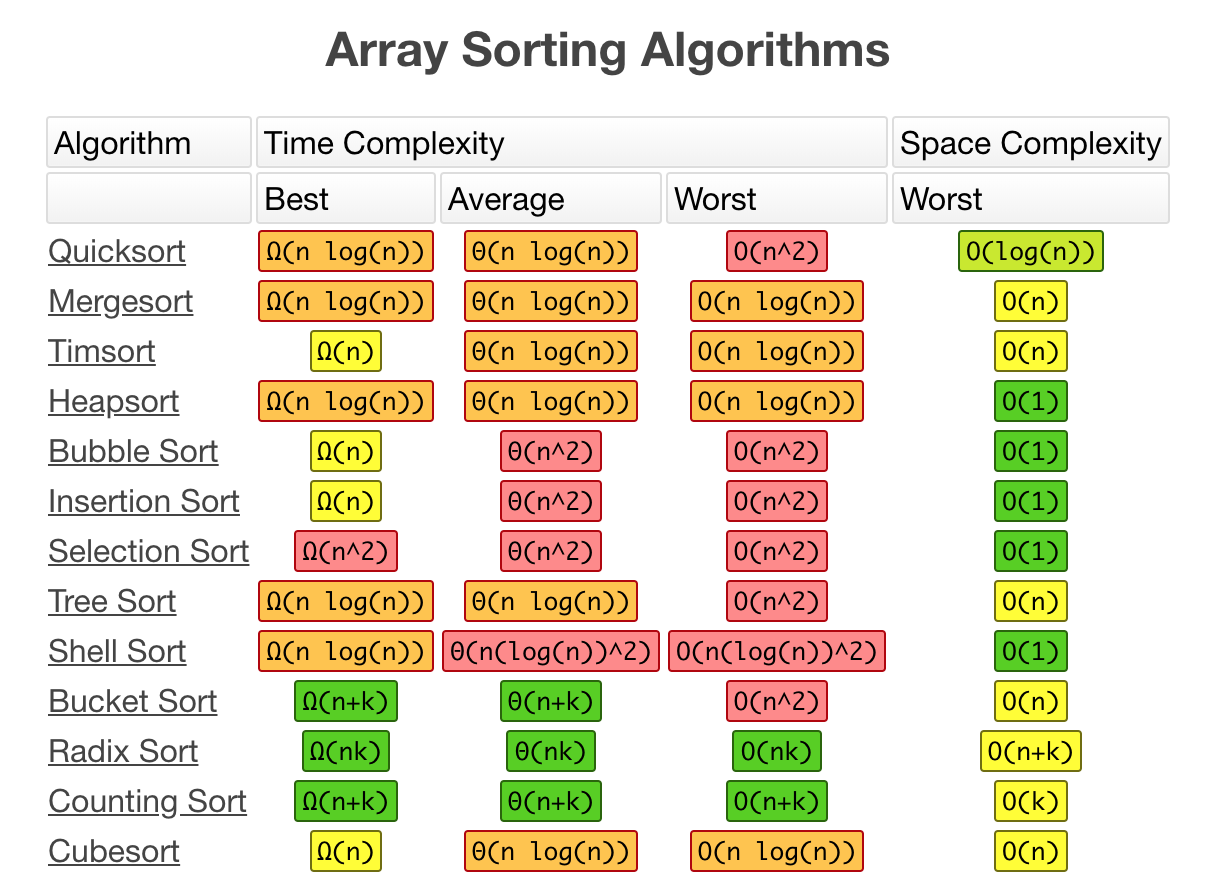
\includegraphics[width=0.5\textwidth]{fig3.png}
  \end{center}

  \item There is a binary tree with height 4 and exactly 16 nodes. \\ 
  \textbf{True} \\
  \ans The height of a rooted tree is the height of its root. That is, the height of a tree is the number of edges in a longest possible path, going away from the root, that starts at the root and ends at a leaf.

  \item The number of exchanges performed by Selection Sort in the worst case when sorting an $n$-element sequence is O($n$). \\
  \textbf{True} \\
  \ans One of the simplest sorting algorithms works as follows: First, find the smallest item in the array and exchange it with the first entry (itself if the first entry is already the smallest). Then, find the next smallest item and exchange it with the sec- ond entry. Continue in this way until the entire array is sorted. This method is called selection sort because it works by repeatedly selecting the smallest remaining item.

  \item A Radix Sort can sort any $n$-element sequence of 9-digit (decimal) integers in O($n$) steps. \\ 
  \textbf{True} \\
  \ans O($kn$) = O($9n$) = O($n$)

  \item  $43n^3\log n + 27n^2 \log \log n$ is O($n^3$) \\
  \textbf{False} \\
  \ans We cannot discard $\log n$ from $43n^3\log n$. This equation is O($n^3\log n$).

  \item Insertion Sort is a stable sort. \\
  \textbf{True} \\
  % \ans
  % \begin{center}
  %   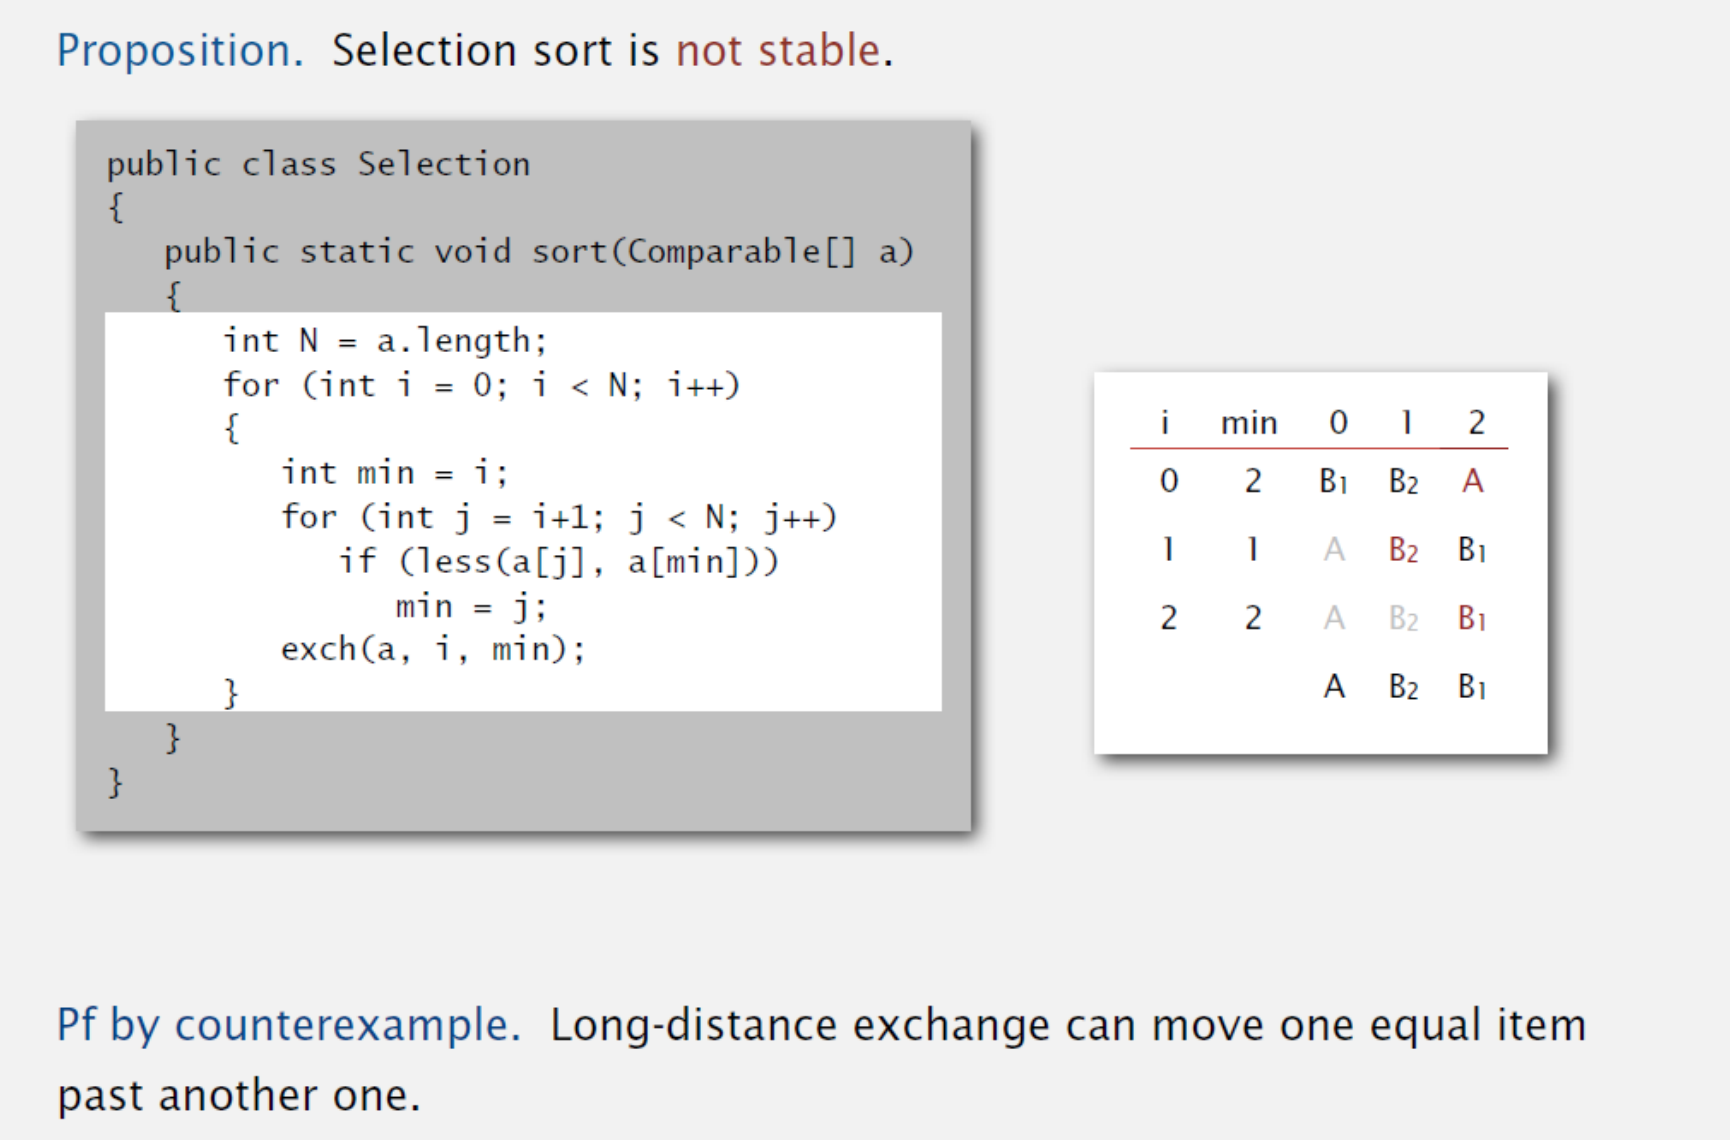
\includegraphics[width=0.7\textwidth]{fig4.png}
  % \end{center}

\end{enumerate}

\section*{Multiple-Choice}
\begin{question}{8}
You are given a list of 800 student names in alphabetical order together with
which class section they are in. The section is a number between 1 and 6. You wish to form
a list of the names in order by section number and alphabetized within each section. Which
of these algorithms would be most efficient to perform this task? 

\begin{enumerate}[label=\alph*]
  \item \textbf{Bucket Sort.}
  \item Heap Sort.
  \item Quicksort.
  \item Priority Queue.
  \item Radix Sort.
\end{enumerate}
\ans Bucket sort, or bin sort, is a sorting algorithm that works by distributing the elements of an array into a number of buckets. Each bucket is then sorted individually, either using a different sorting algorithm, or by recursively applying the bucket sorting algorithm.
\end{question}

\begin{question}{9}
Which one of these data structures uses the “swim up” and “sink down”
operations?

\begin{enumerate}[label=\alph*]
  \item Queue.
  \item Stack.
  \item \textbf{Heap.}
  \item Hash table.
  \item Binary Search Tree.
\end{enumerate}

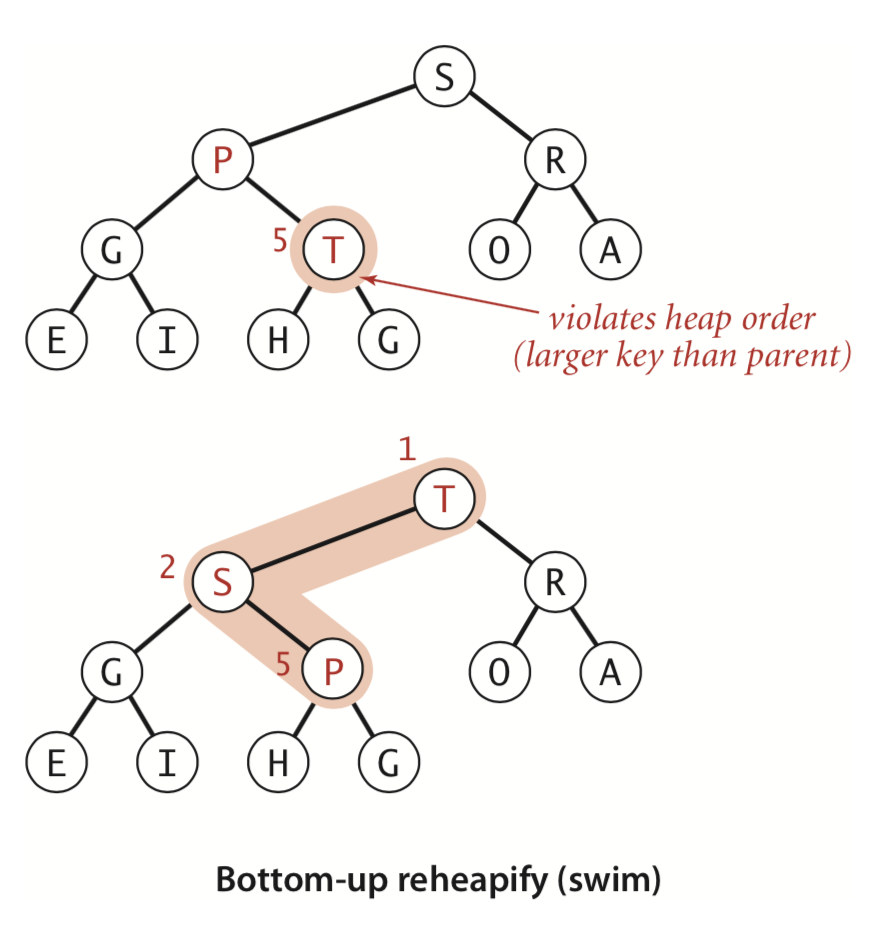
\includegraphics[width=0.5\textwidth]{fig5.png}
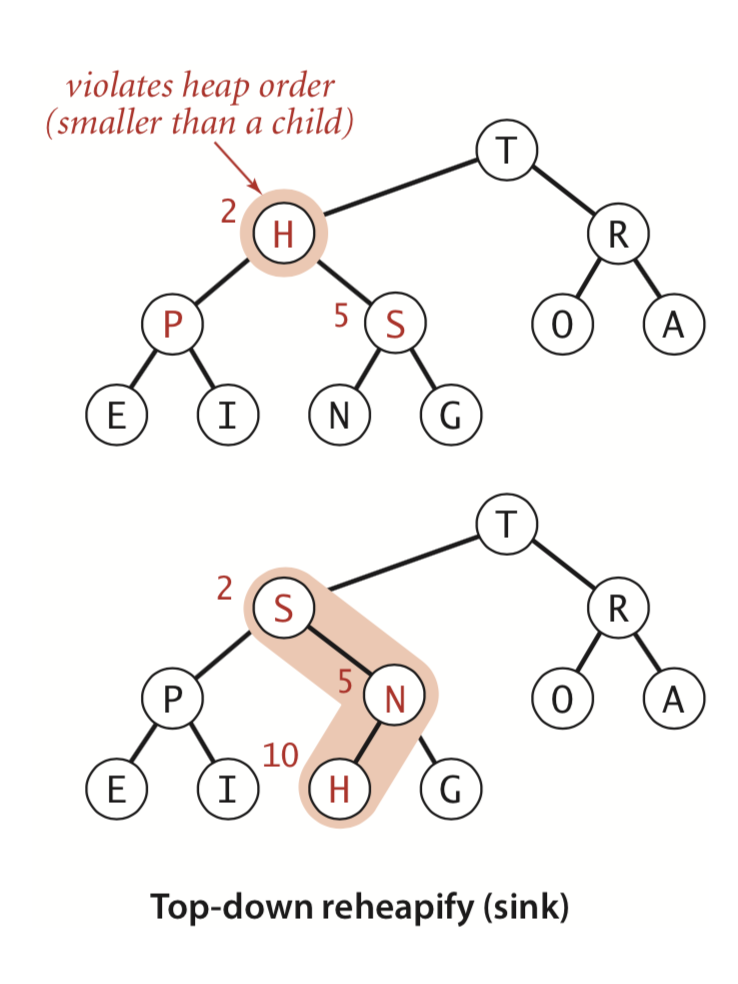
\includegraphics[width=0.5\textwidth]{fig6.png}

\end{question}

\begin{question}{10}
Which of the following functions would be the best hash function for Social
Security Numbers (which are 9-digit integers) to use for a hash table of size about 1000 with linear probing?

\begin{enumerate}[label=\alph*]
  \item The sum of the digits.
  \item The first three digits.
  \item The middle three digits.
  \item The three digit number formed from the first, fourth and seventh digits.
  \item \textbf{The SSN$\%p$, where $p$ is a prime number near 1000.}
\end{enumerate}

\end{question}

\begin{question}{11}
If $3N^3 + 2N^2 + 6N \log N − 3 ∼ N^e$, then $e =$

\begin{enumerate}[label=\alph*]
  \item 1.
  \item 2.
  \item 3.
  \item 4.
  \item \textbf{There is no integer e that makes this statement true.}
\end{enumerate}
\ans Correct $\sim$ notation will be $\sim 3N^3$.

\end{question}


\section*{Part II.}

\begin{question}{12}
A small Hash table uses linked lists and Hashcode$(x) = x\%7$ to store integers $x$. Show the
contents of the Hash table after these operations.

\begin{itemize}
  \item Insert(13) Hash: 6
  \item Insert(16) Hash: 2
  \item Insert(2) Hash: 2
  \item Insert(9) Hash: 2
  \item Delete(16) Hash: 2
  \item Insert(6) Hash: 6
  \item Delete(13) Hash: 6
\end{itemize}
\ans \\
\begin{tabular}{c|c}
Hashcode & Content \\ \hline
0        &         \\
1        &         \\
2        & 2, 9    \\
3        &         \\
4        &         \\
5        &         \\
6        & 6      
\end{tabular}

\end{question}

\begin{question}{13}
Give the output of the following series of Priority Queue operations. The Priority Queue
has space for 100 elements and is initially empty. (The output may be an exception or void.
If void, you must write “void” for the output.) \\
\ans \\
\begin{tabular}{c|c|c}
\hline
Operation  & Output & Contents (ordered) \\ \hline
insert(9)  & void   & 9                  \\
insert(13) & void   & 9, 13              \\
insert(19) & void   & 9, 13, 19          \\
insert(2)  & void   & 2, 9, 13, 19       \\
max()      & 19     & 2, 9, 13, 19       \\
insert(7)  & void   & 2, 7, 9, 13, 19    \\
insert(1)  & void   & 1, 2, 7, 9, 13, 19 \\
size()     & 6      & 1, 2, 7, 9, 13, 19 \\
delMax()   & 19     & 1, 2, 7, 9, 13     \\
delMax()   & 13     & 1, 2, 7, 9         \\
isEmpty()  & False  & 1, 2, 7, 9         \\
insert(4)  & void   & 1, 2, 4, 7, 9     
\end{tabular}

\end{question}

\begin{question}{14}
A 2-3 Tree has exactly one node, with key value 17. Draw the tree after the following
operations are performed on it.

\begin{enumerate}
  \item insert(2)
  \item insert(3)
  \item insert(29)
  \item insert(25)
  \item insert(35)
  \item deleteMin()
  \item insert(36)
  \item insert(30)
  \item insert(26)
  \item delete(29)
  \item delete(17)
\end{enumerate}
\ans
\begin{center}
  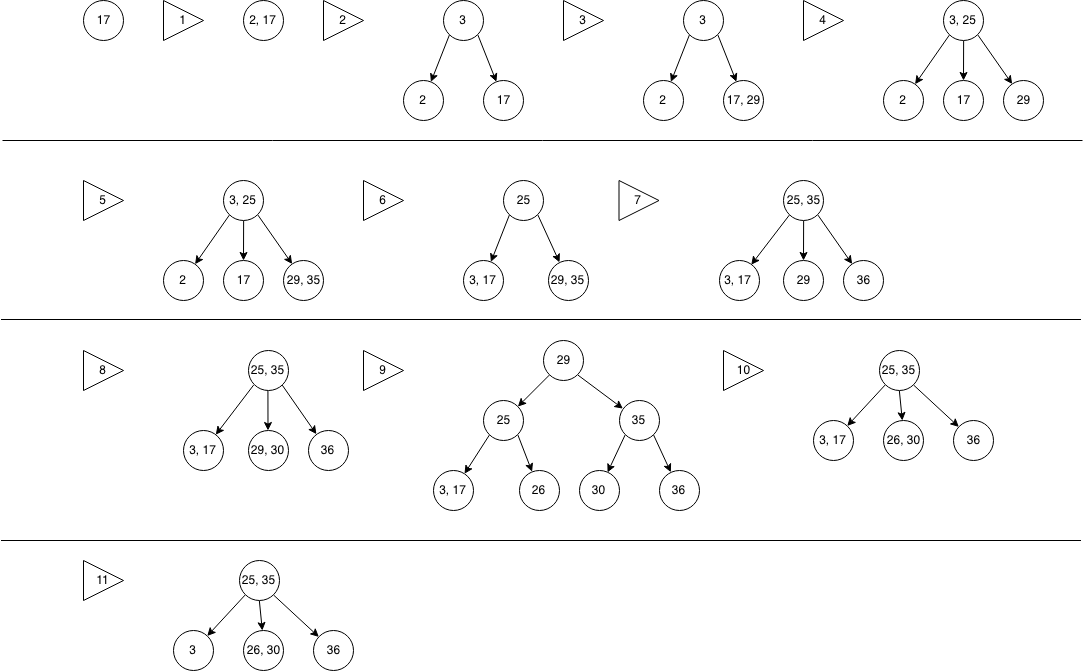
\includegraphics[width=\textwidth]{fig7.png}
\end{center}

\end{question}


\begin{question}{15}
For each of the following sorting algorithms, give the requested running times using big-Oh
notation. There are N items to sort. Assume that a single comparison takes constant time.
Omit the cases labeled “Omit”. \\

\ans \\
\begin{tabular}{|c|c|c|c|}
\hline
\textbf{Algorithm}                            & \textbf{Best Case} & \textbf{Average Case} & \textbf{Worst Case} \\ \hline
Heap Sort on a Priority Queue based on a Heap & $n \log n$         & $n \log n$            & Omit                \\ \hline
Selection Sort as in class                    & Omit               & $n^2$                 & $n^2$               \\ \hline
Insertion Sort as in class                    & $n$                & Omit                  & $n^2$               \\ \hline
Merge Sort as in class                        & $n \log n$         & $n \log n$            & Omit                \\ \hline
In Place QuickSort (not Randomized)           & $n \log n$         & Omit                  & $n^2$               \\ \hline
\end{tabular}
\end{question}

\begin{question}{16}
Order the following 16 functions by big-Oh notation, with the slowest-growing one (as $n →
∞$) at the top and the fastest-growing one (as $n → ∞$) at the bottom. List on the same line
all functions that are big-Theta of one another. Here “$\log x$” means “$\log_2 x$”.

\begin{center}
  \begin{tabular}{llll}
  $8n \log n$  & $4^n$        & $\log \log n$ & $2^{\log n} = n$   \\
  $2^{1000}$   & $2^n$        & $n^{0.01}$    & $6n^{3/2}$     \\
  $2^{2^n}$    & $3^{\log n}$ & $n/100$       & $\sqrt{\log n}$\\
  $3 \sqrt{n}$ & $53n$        & $1/n$         & $(\log n)^2$      
  \end{tabular}
\end{center}

\ans \\
Slowest-growing one (as $n → ∞$).
\begin{enumerate}
  \item $1/n$
  \item $2^{1000}$
  \item $\log \log n$
  \item $n^{0.01}$
  \item $\sqrt{\log n}$
  \item $(\log n)^2$
  \item $3 \sqrt{n}$
  \item $2^{\log n} = n$, $n/100$, $53n$
  \item $6n^{3/2}$
  \item $3^{\log n}$
  \item $8n \log n$
  \item $2^n$
  \item $4^n$
  \item $2^{2^n}$
\end{enumerate}
Fastest-growing one (as $n → ∞$).

\end{question}

\end{document}
